% 归档自 sections/01_dream_start.tex「CLion 格式化：括号内加空格」一节 (2026-07-23)
% 配图仍在 image/ 目录: CLion 括号内空格配置.png / CLion 表达式括号内空格.png / CLion 函数调用括号内空格.png

		\subsection{CLion 格式化：括号内加空格}

		\textbf{Settings} → \textbf{Editor} → \textbf{Code Style} → \textbf{C/C++} → \textbf{Spaces} 标签下，下面三个开关都要勾，单独勾任何一个都不彻底——分别覆盖函数声明形参括号、表达式 grouping 括号、函数调用 / 初始化括号。

		\begin{itemize}
			\item \textbf{Within} → \textbf{Parentheses}：函数声明的形参括号内壁加空格，\mintinline{cpp}{circle_relation( const Circle<T> &a, const Circle<T> &b )}。
			\item \textbf{In expressions} → \textbf{Within parentheses}：表达式 grouping 括号，\mintinline{cpp}{(b - a) / 2} → \mintinline{cpp}{( b - a ) / 2}。
			\item \textbf{Within parentheses in function call and initialization}：函数调用和构造调用，\mintinline{cpp}{foo(a, b)} → \mintinline{cpp}{foo( a, b )}、\mintinline{cpp}{Circle<DB>(I, r)} → \mintinline{cpp}{Circle<DB>( I, r )}。
		\end{itemize}

		\begin{center}
			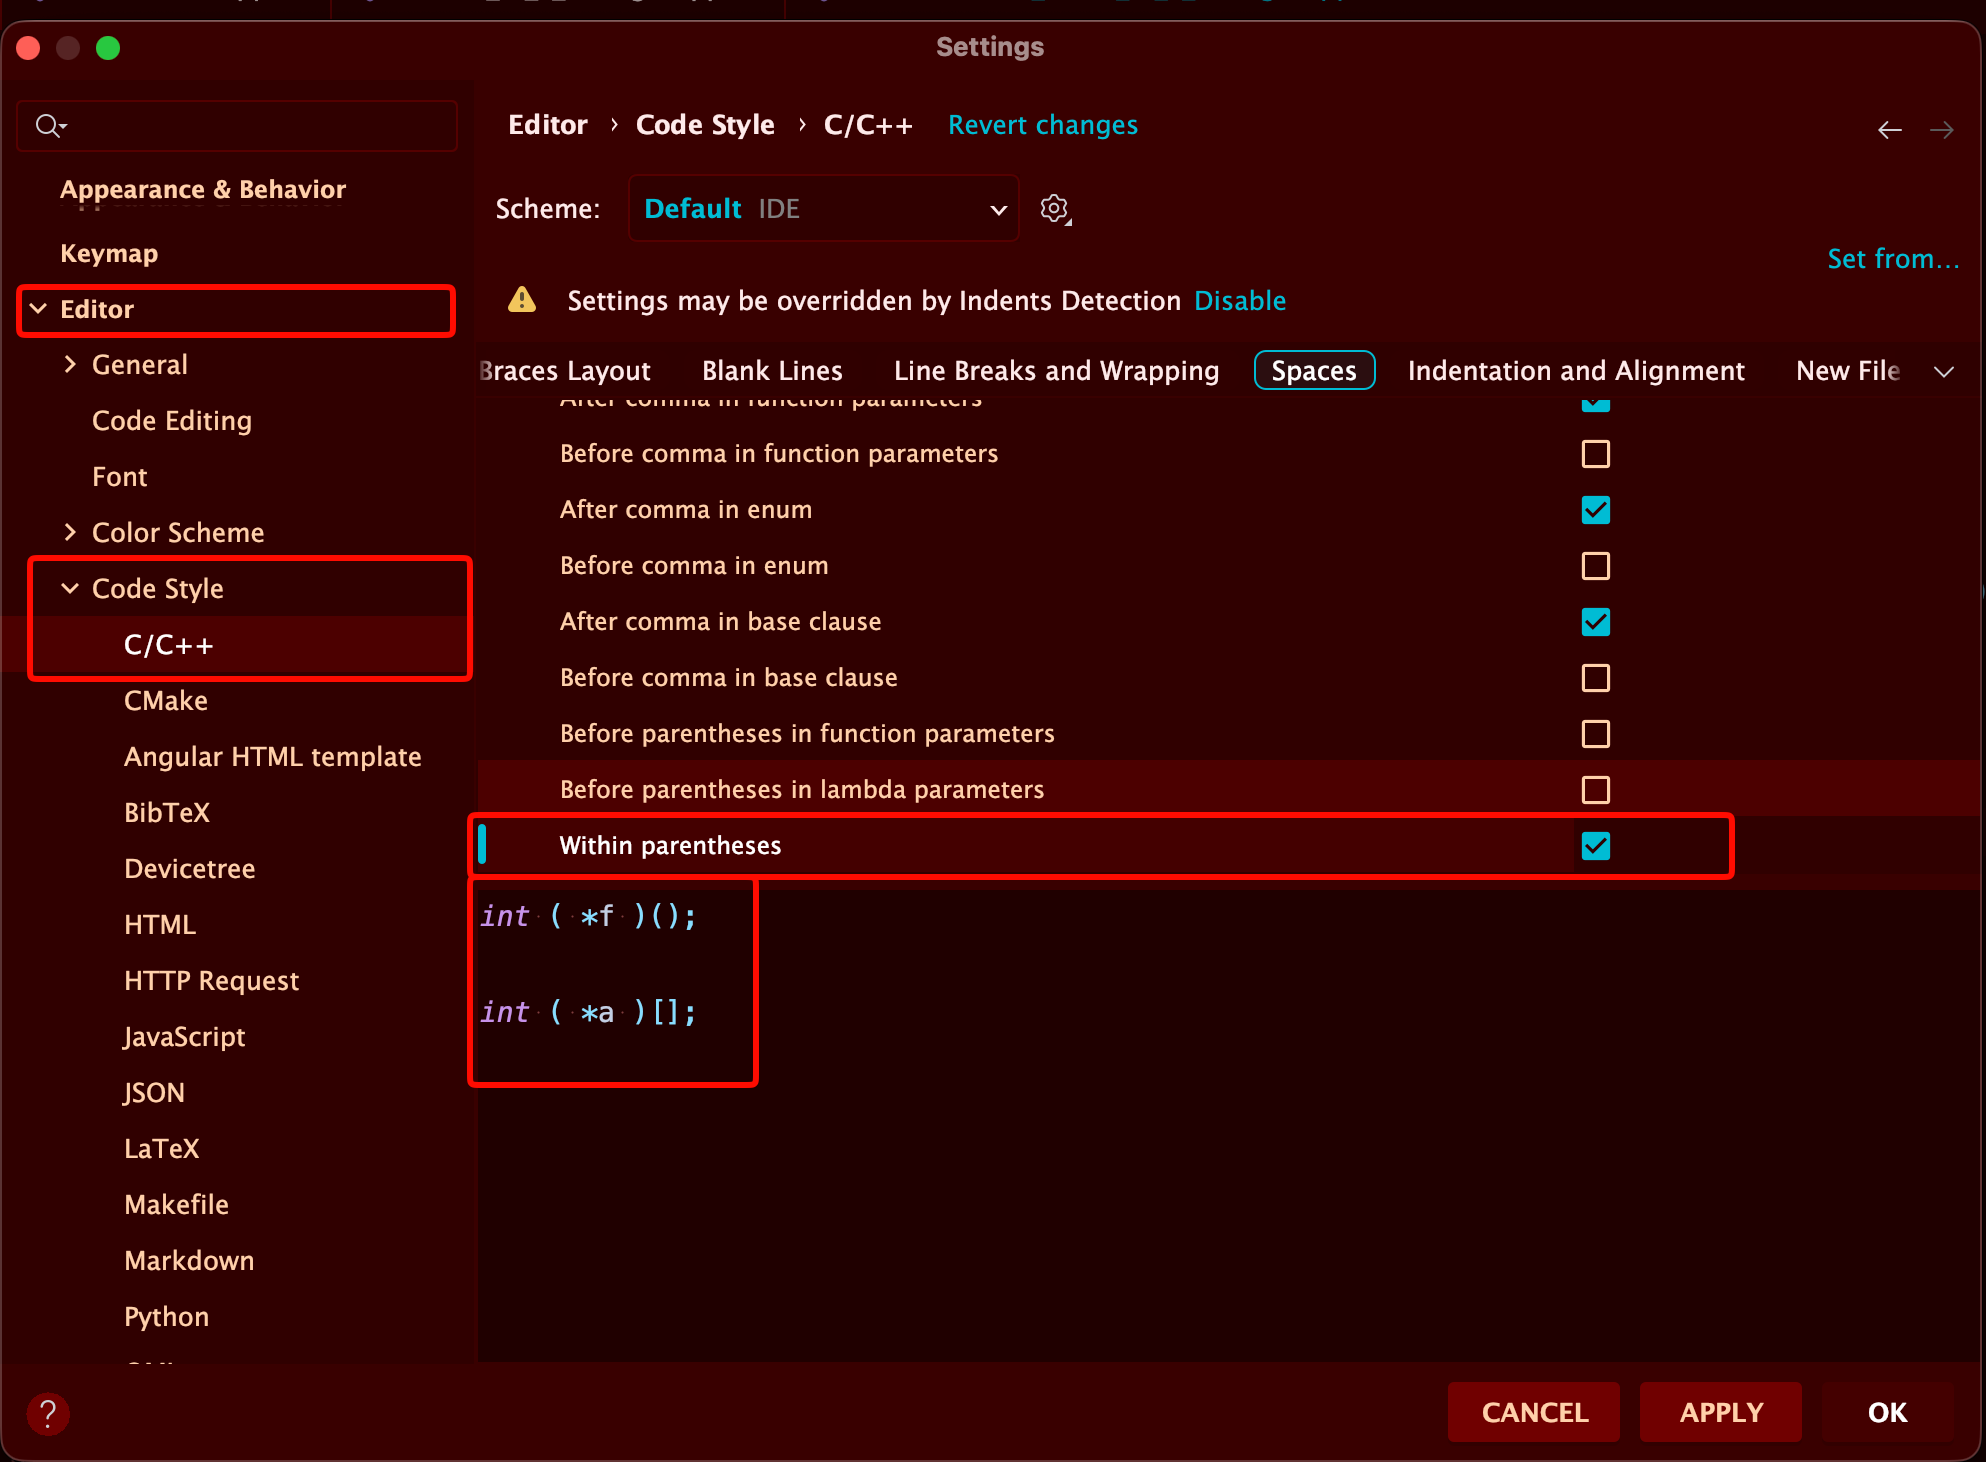
\includegraphics[width=\linewidth]{image/CLion 括号内空格配置.png}
		\end{center}

		\begin{center}
			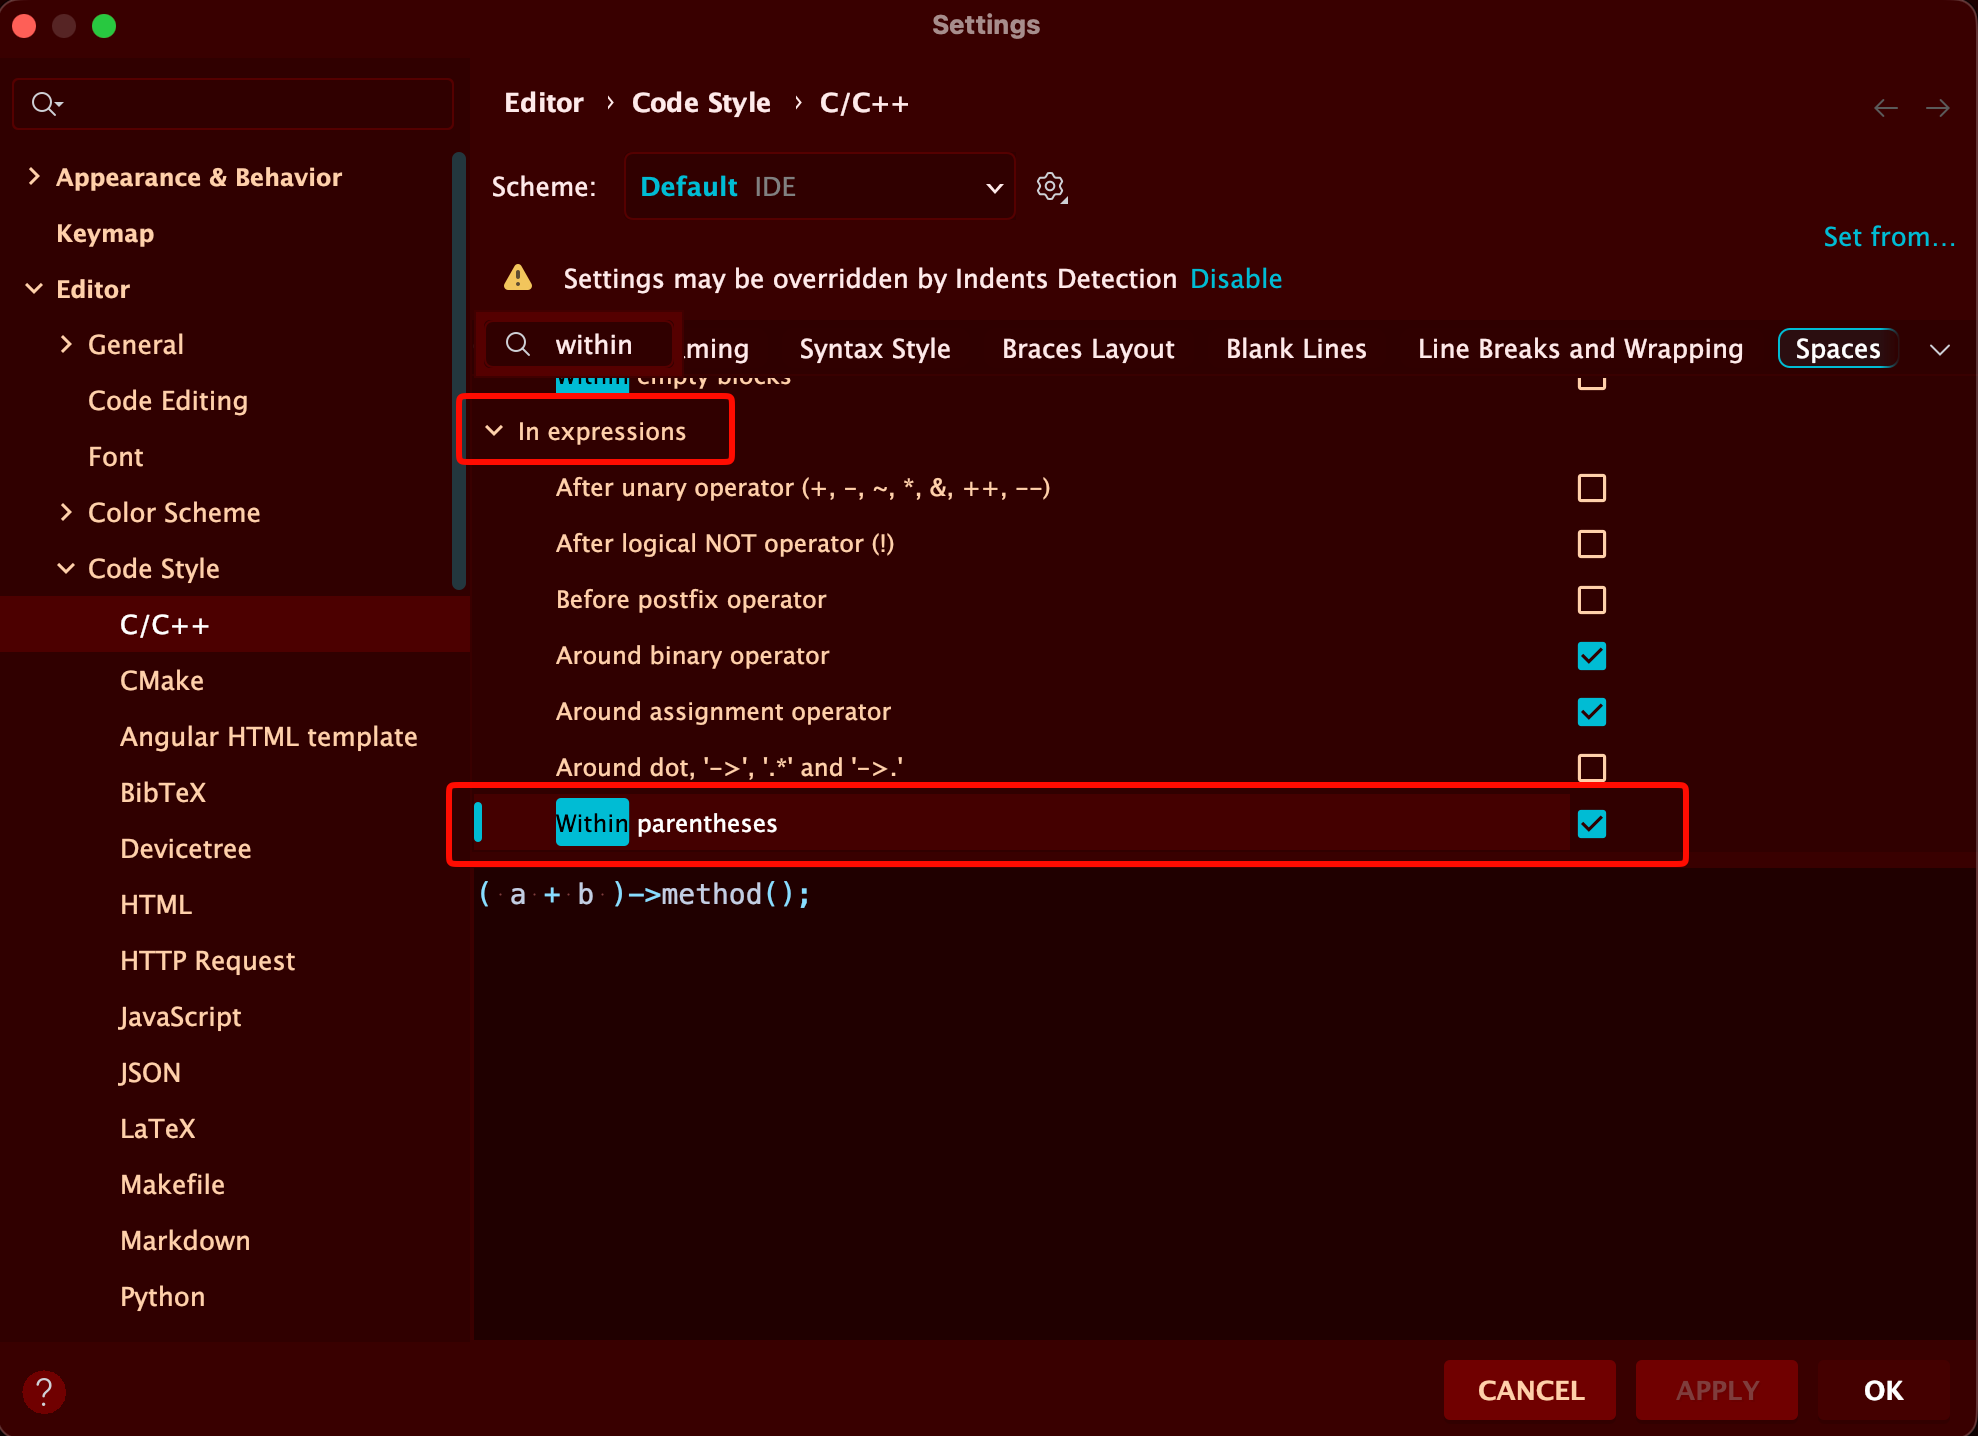
\includegraphics[width=\linewidth]{image/CLion 表达式括号内空格.png}
		\end{center}

		\begin{center}
			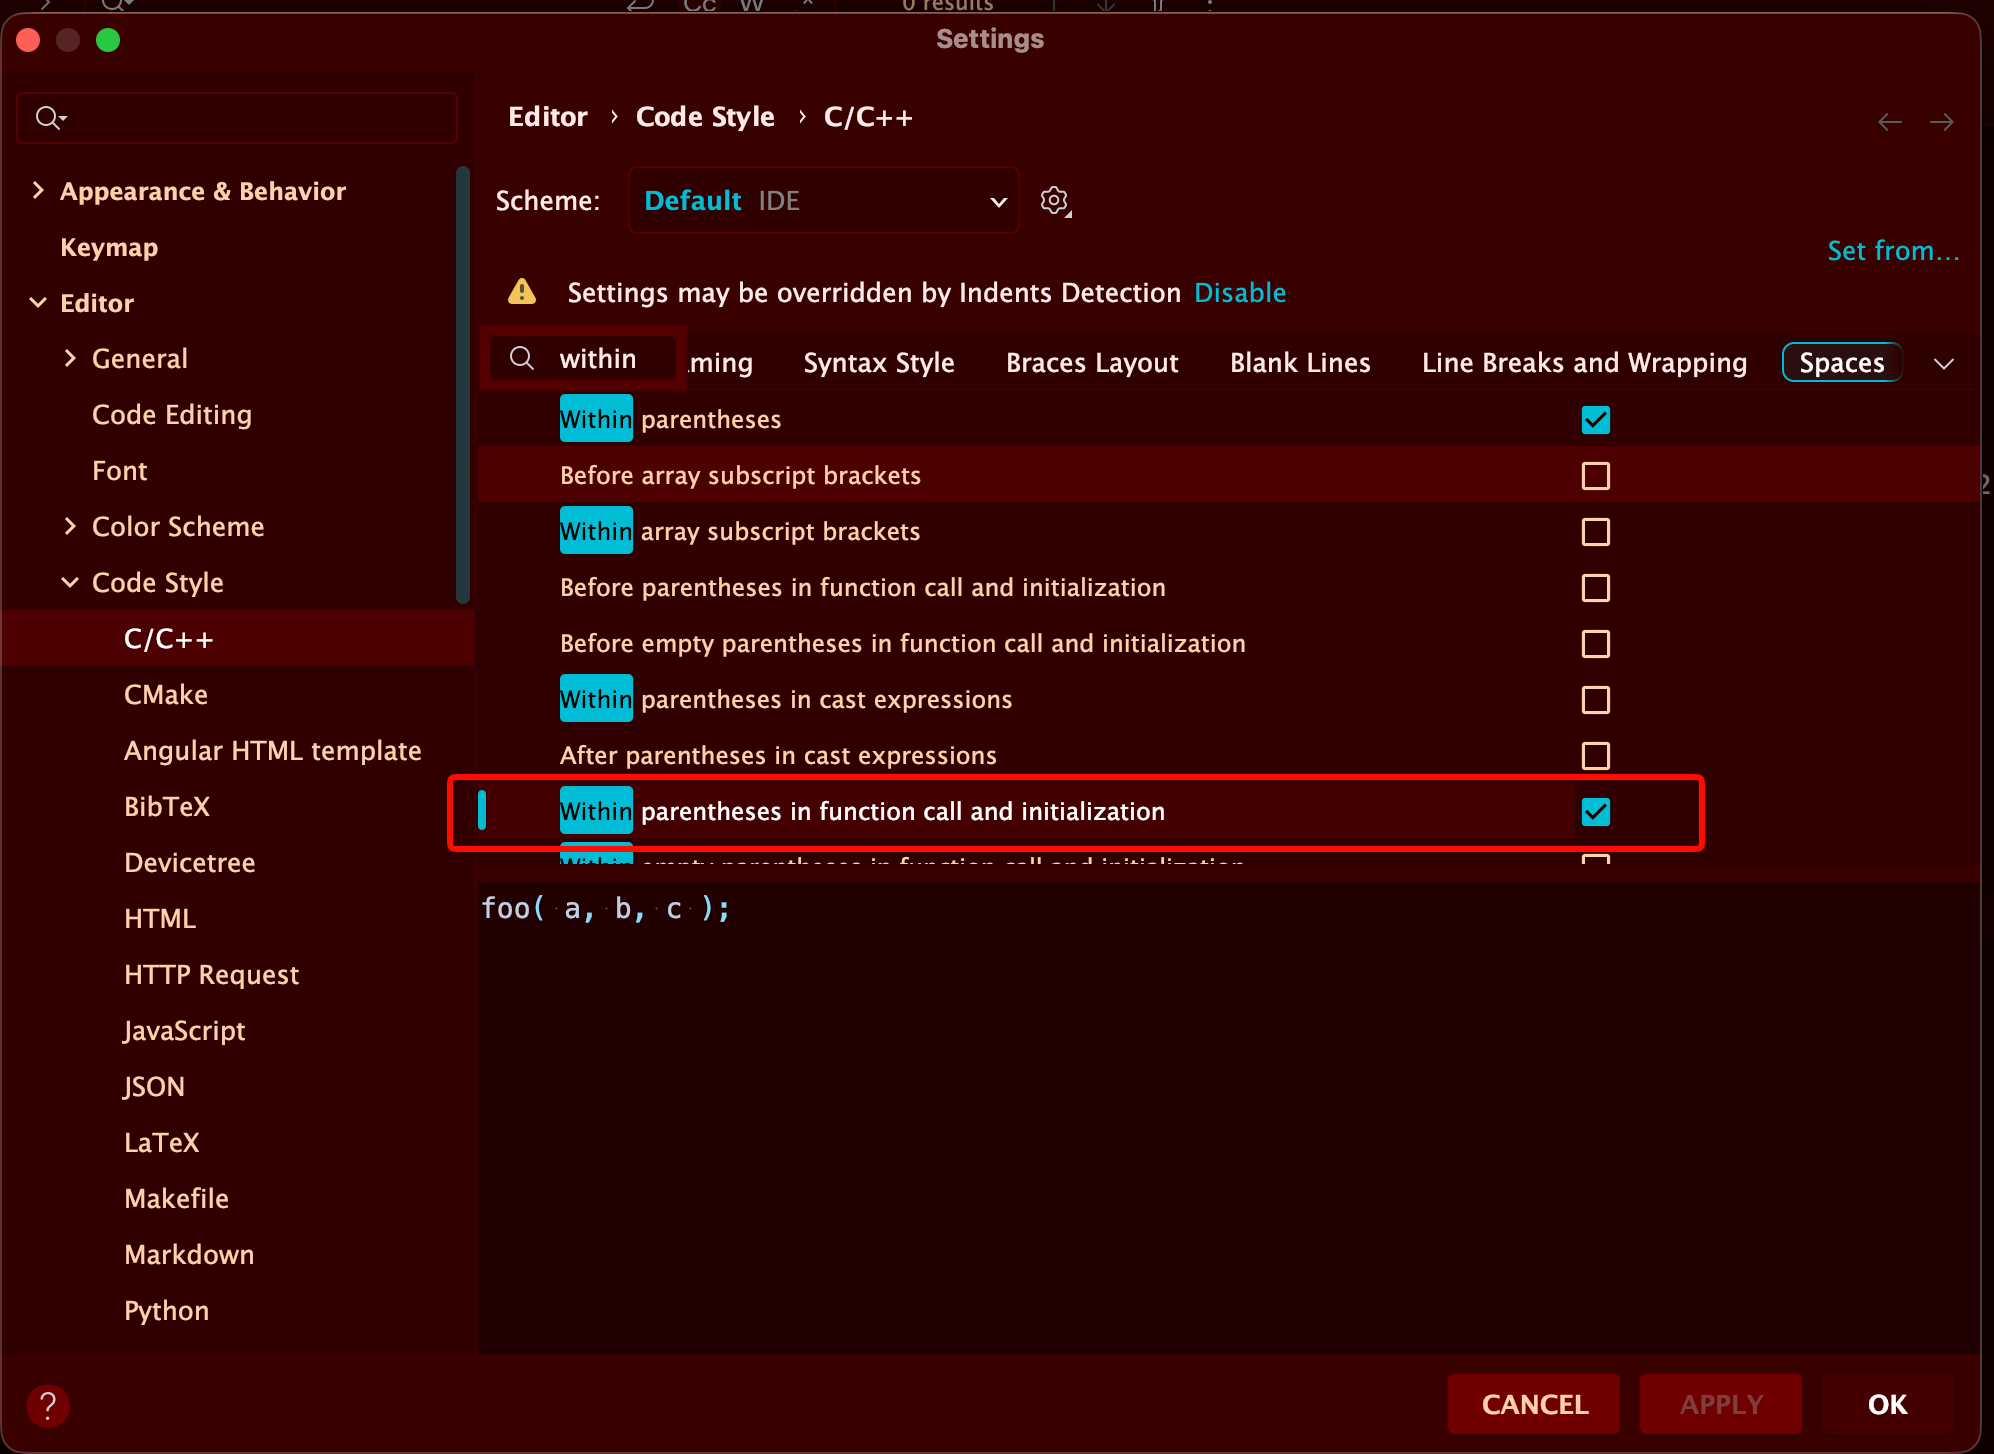
\includegraphics[width=\linewidth]{image/CLion 函数调用括号内空格.png}
		\end{center}
